\section{Discussion}
\label{sec:Discussion}
%include figure of downlinked data
%maybe some sort of figure from astrobiology?
%general discussion introduction, go in depth for other sections while referencing figures.
%since no biology results, we need to go into failure analyze mode and find out what can be done better in the future.
\begin{figure}[h!]
	\begin{center}
		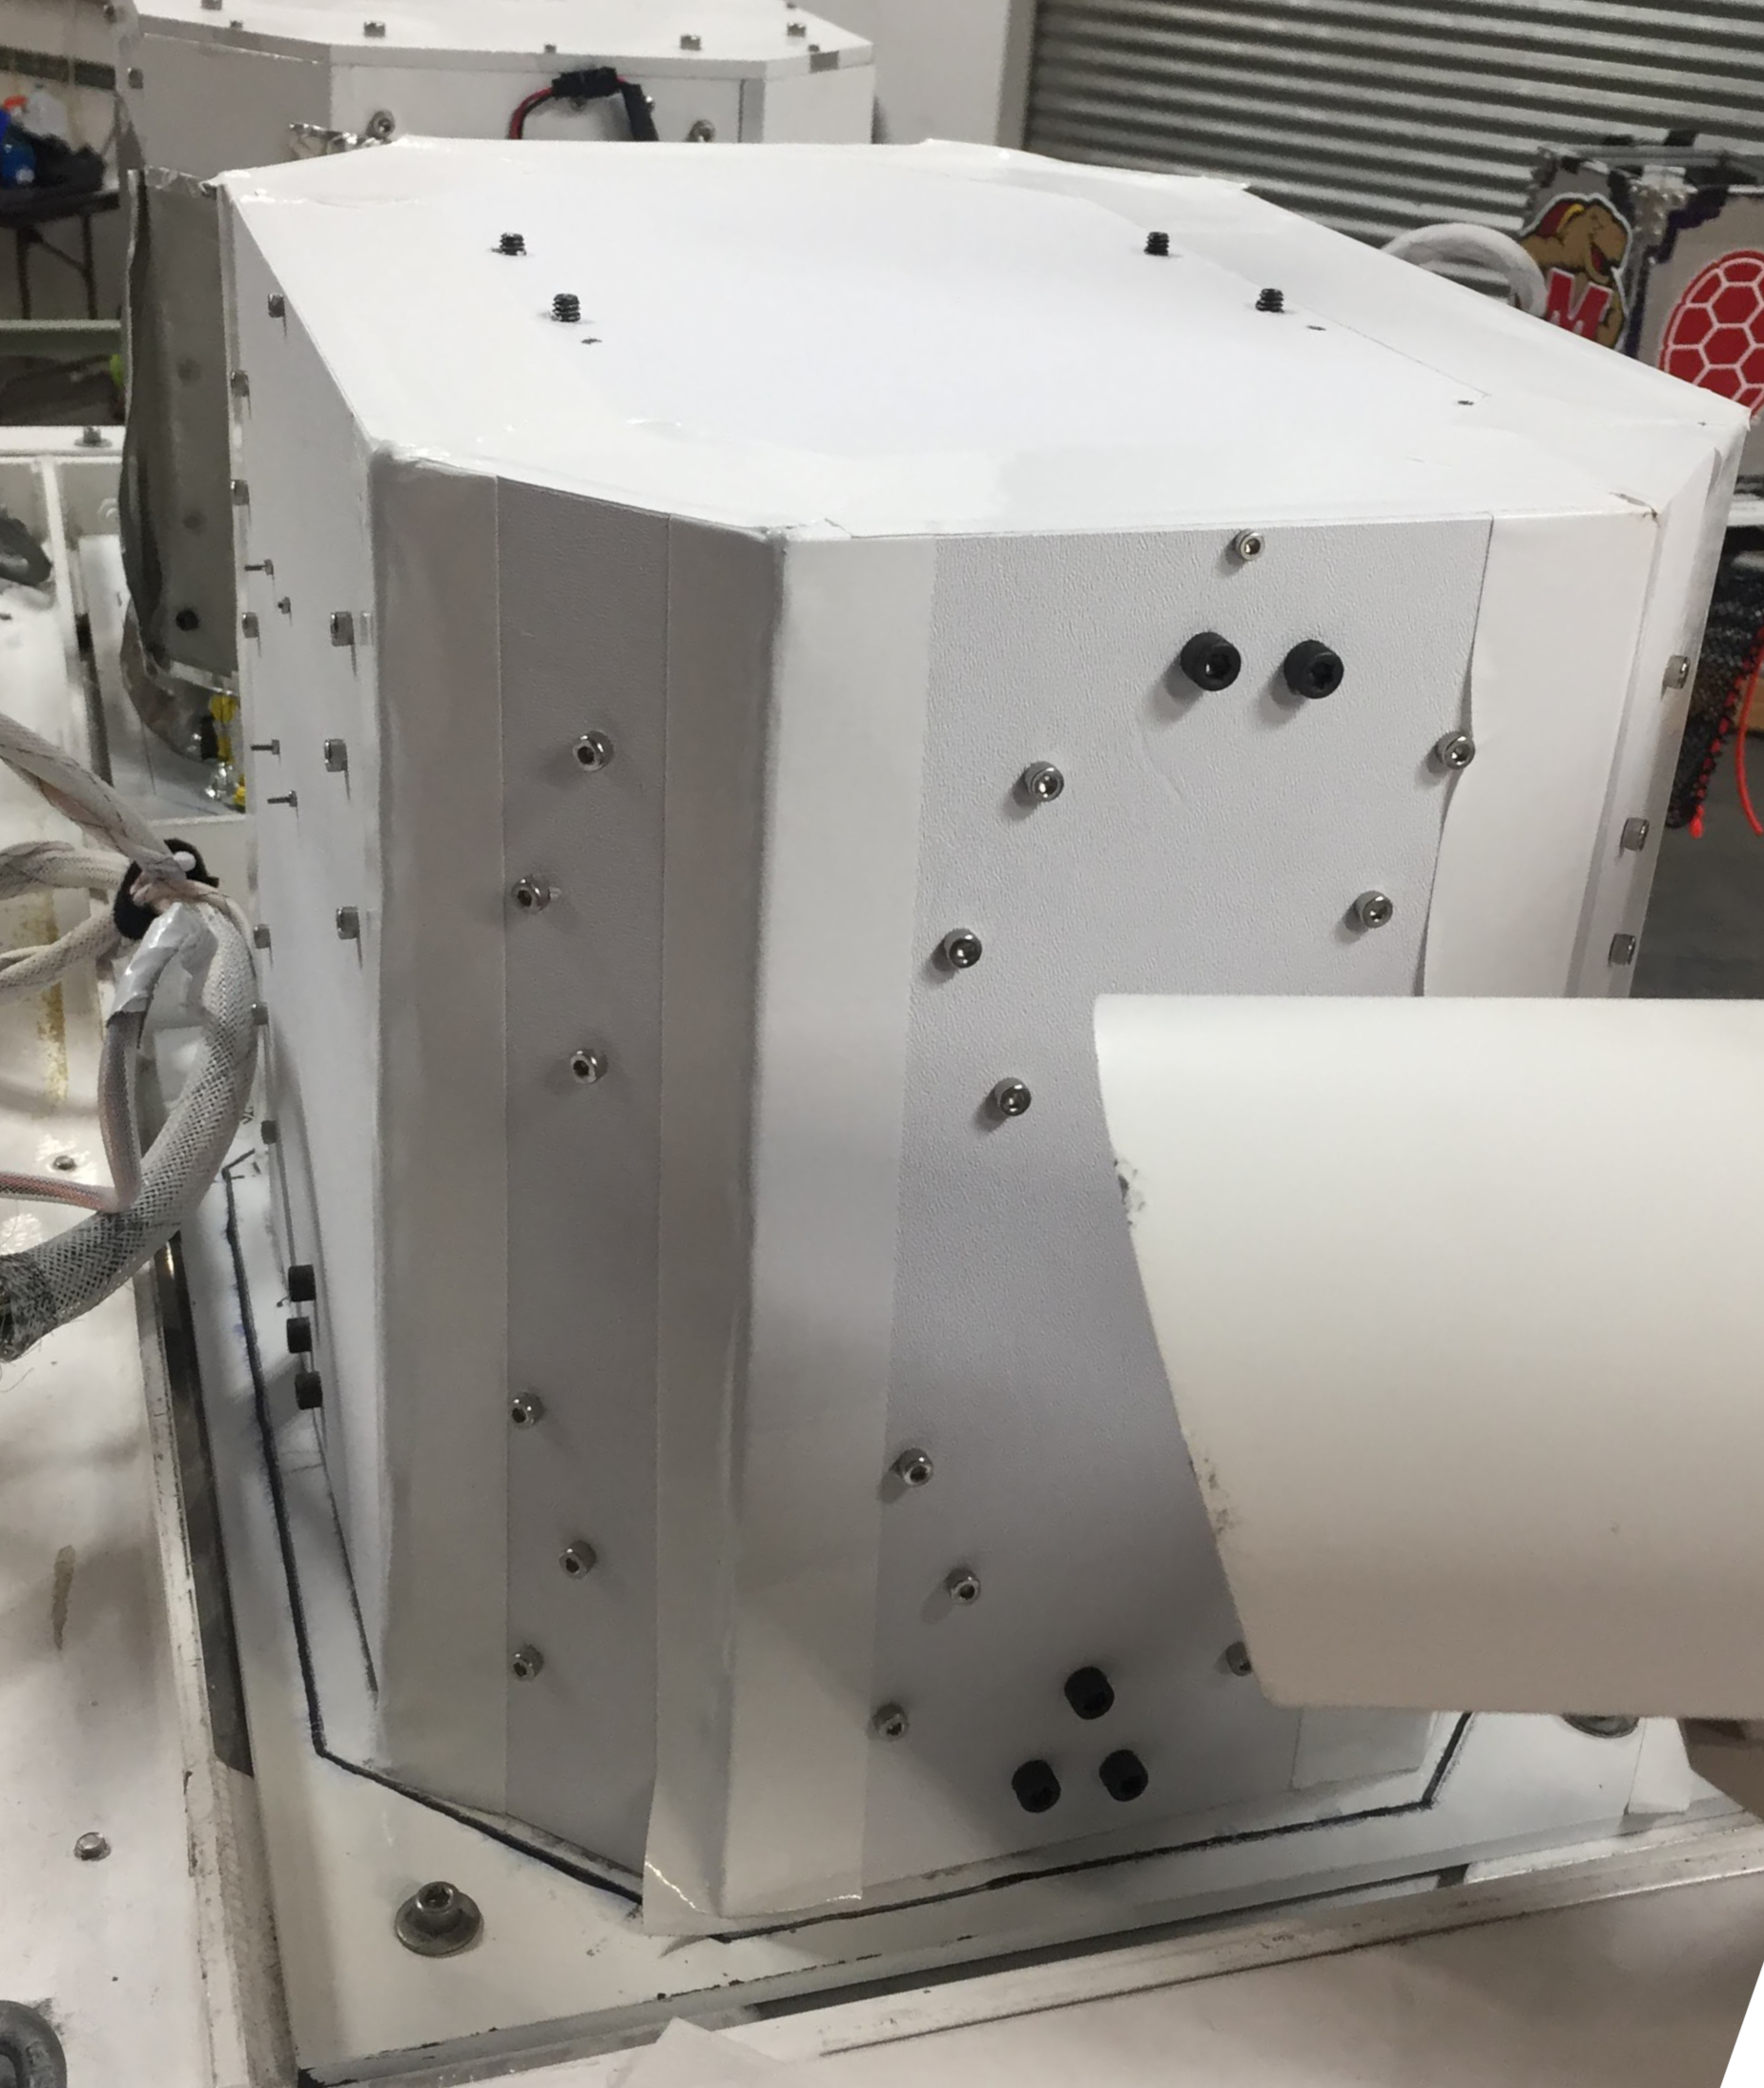
\includegraphics[width=70 mm, scale=1]{figures/payload_integrated.JPG}
		\caption{Final payload integrated and ready for flight}
		\label{fig:payload_int}
	\end{center}
\end{figure}

SORA 2.0 was safely recovered after landfall.  Thanks to the outer shell and build quality, all payload subsystems showed no damage.  
The plastic insulation and reinforced openings aided in maintaining a stable operating temperature inside the payload walls.  
Data and sample integrity both were retrieved successfully.  As seen in Figure \ref{fig:integrationtemps}, data was downlinked without faults or 
missing datum. For astrobiology, samples were recovered safely and sent to be analyzed.  

The only change to the structure that provided a significant advantage during flight was adding duct tape to the corners of the payload walls.  As seen on Figure \ref{fig:payload_int}, the tape covers the corners which allowed for a passive but effective way to manage internal temperature.  The tape was added after initial testing, since the payload would vary in temperature without the tape.  

Overall, the Kydex, flight-proven outershell structure served its purpose once again.  The impact protection, solid construction, and insulation properties of the shell allowed for uninterrupted experiments to take place in the harsh environments of the upper atmosphere.